\documentclass[11pt]{article}
\input{/Users/markwang/.preamble}
\begin{document}



\begin{enumerate}
\item \textbf{Perceptron Algorithm} Training example in 2-dimensional input space with no bias term. Use $t\in \{-1,1\}$. 

\begin{enumerate}
    \item Sketch out the problem in weight space. In particular: draw and label the axes, draw the half-space corresponding to each of the two training examples, and shade the feasible region. (Remember that there is no bias term.) \\
    We can write out equation for 2 hyperplanes in the weight space representing the two training examples. We can specify the half space for the set of possible positive examples as follows
    \[
        w_1 -2w_2 > 0 
        \quad \quad \quad \quad 
        -w_2 < 0
    \]
    Note the half space is denoted by a line with an arrow indicating the side to which we specify as a half space. \\
    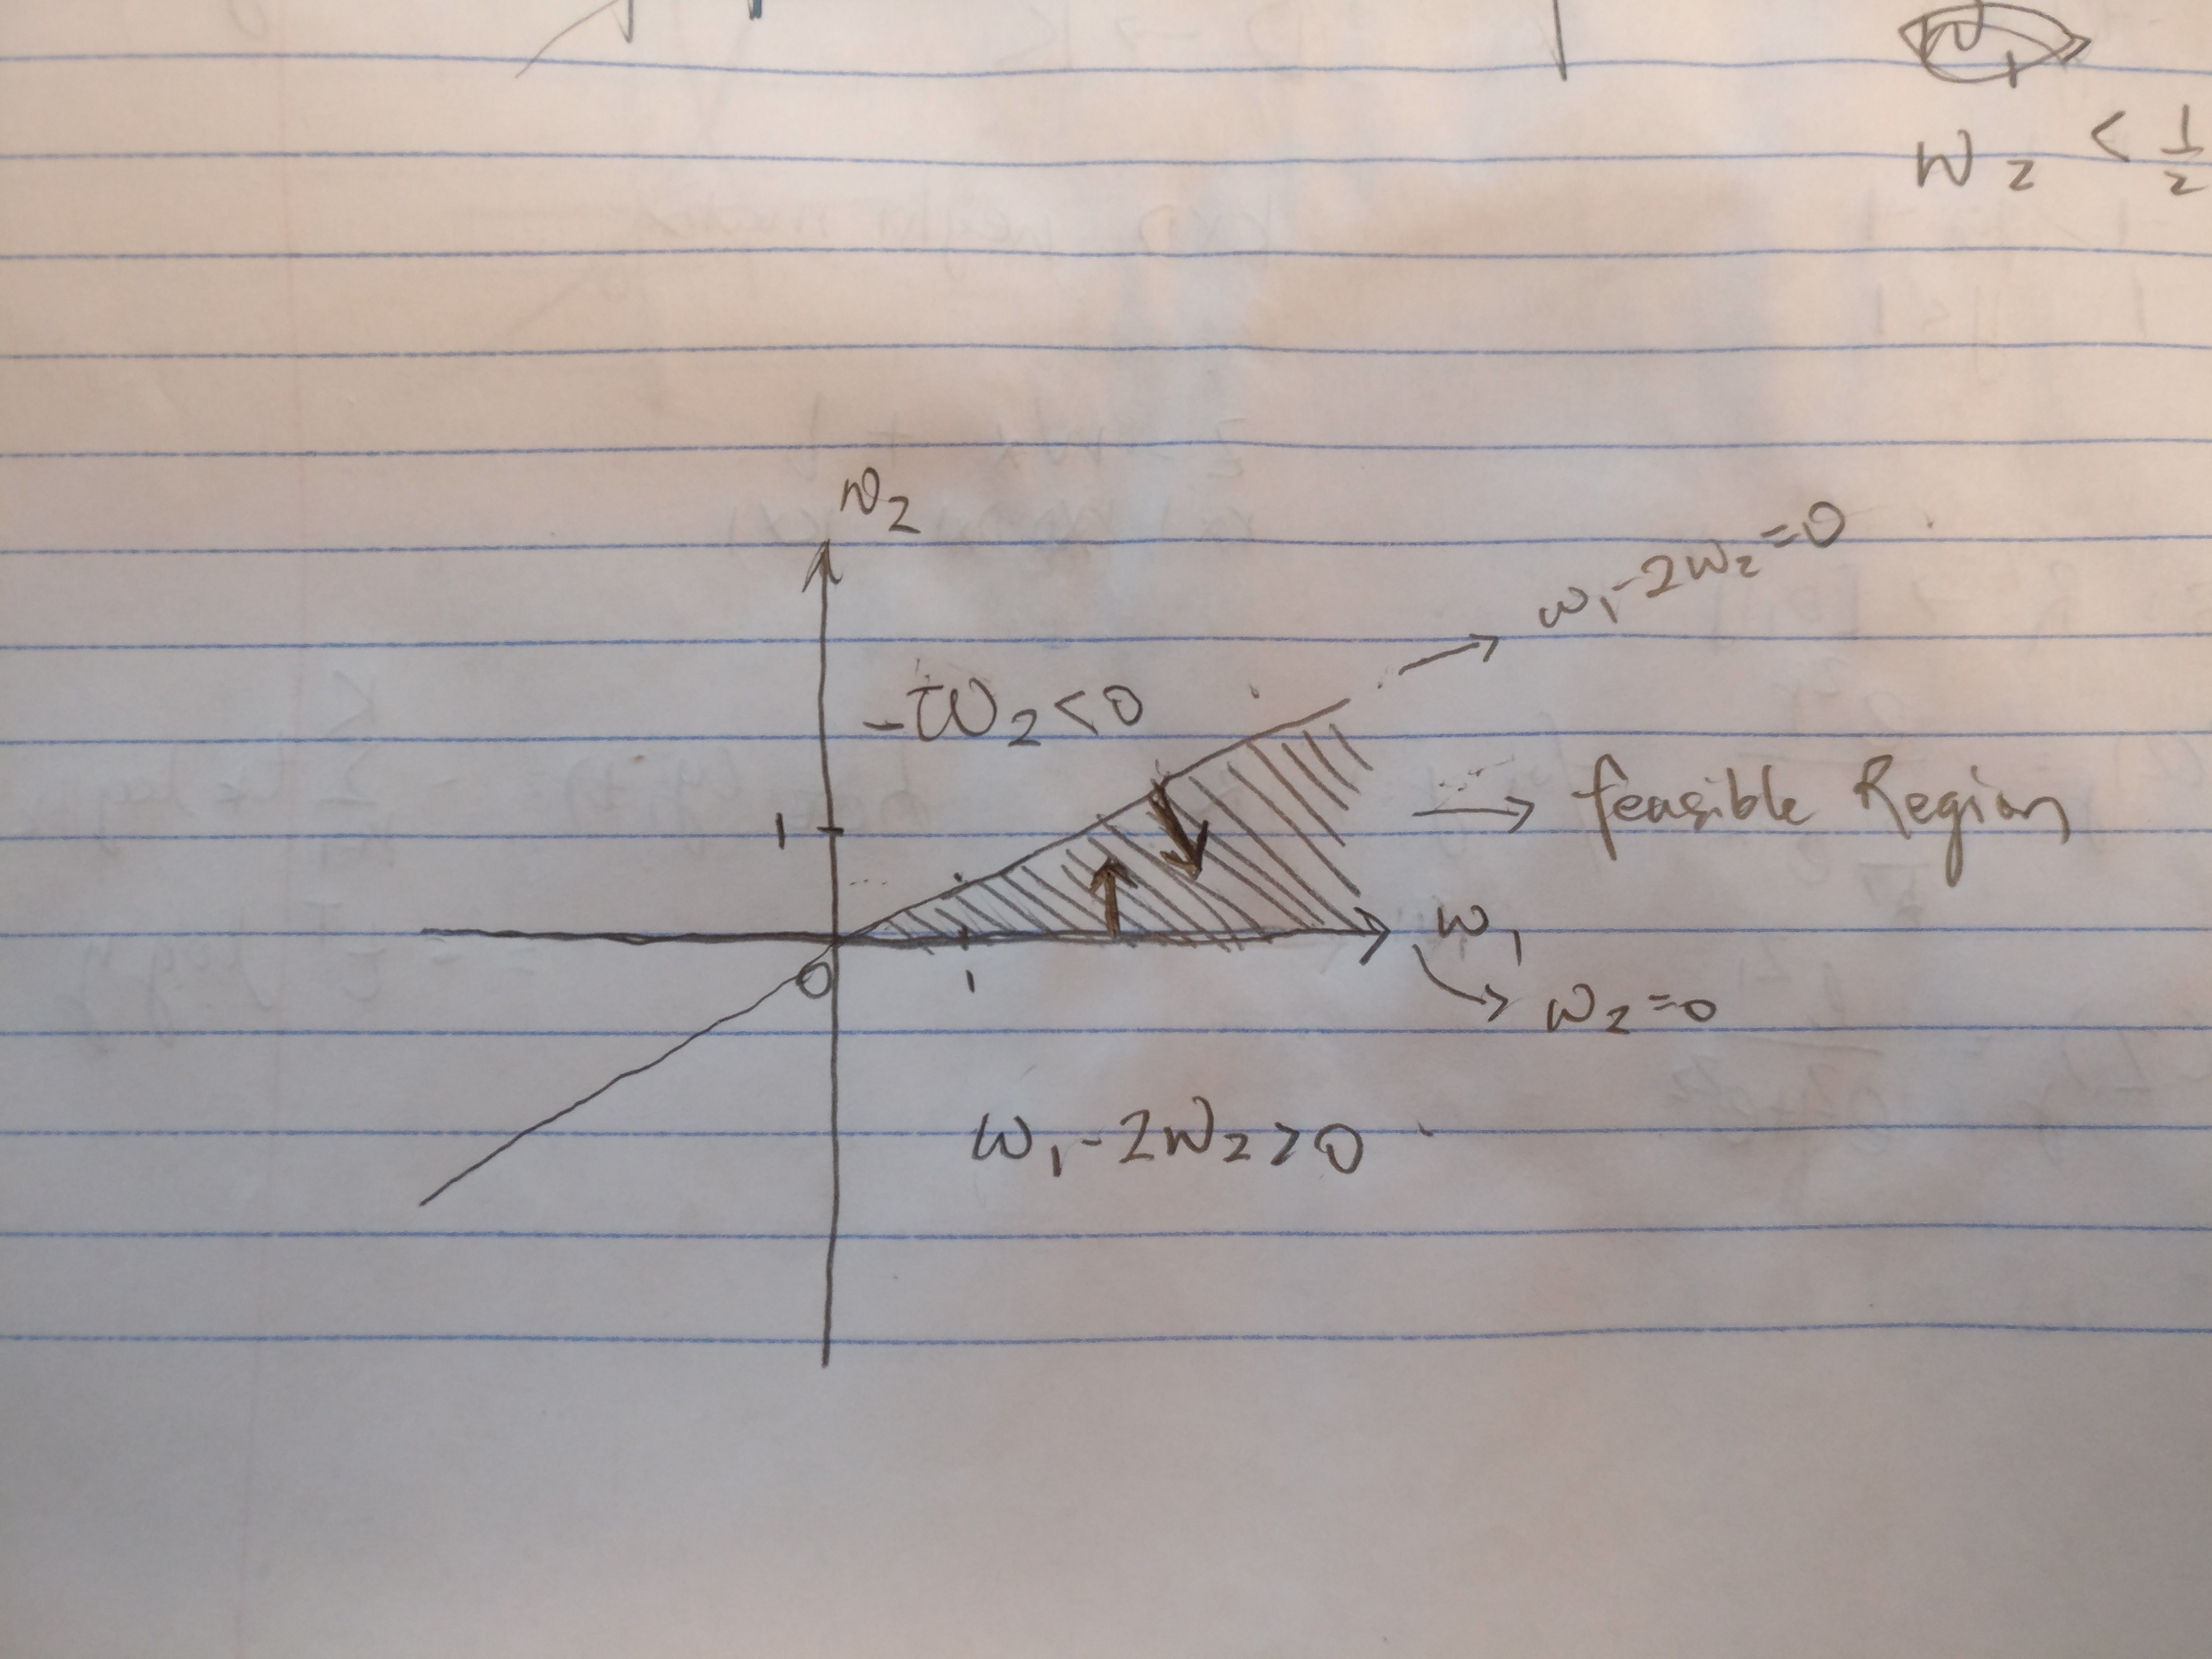
\includegraphics[width=10cm]{weightspace.jpg}
    \item  Simulate the perceptron algorithm by hand, starting from the initial weights w1 = 0, w2 = −2. \\ 
    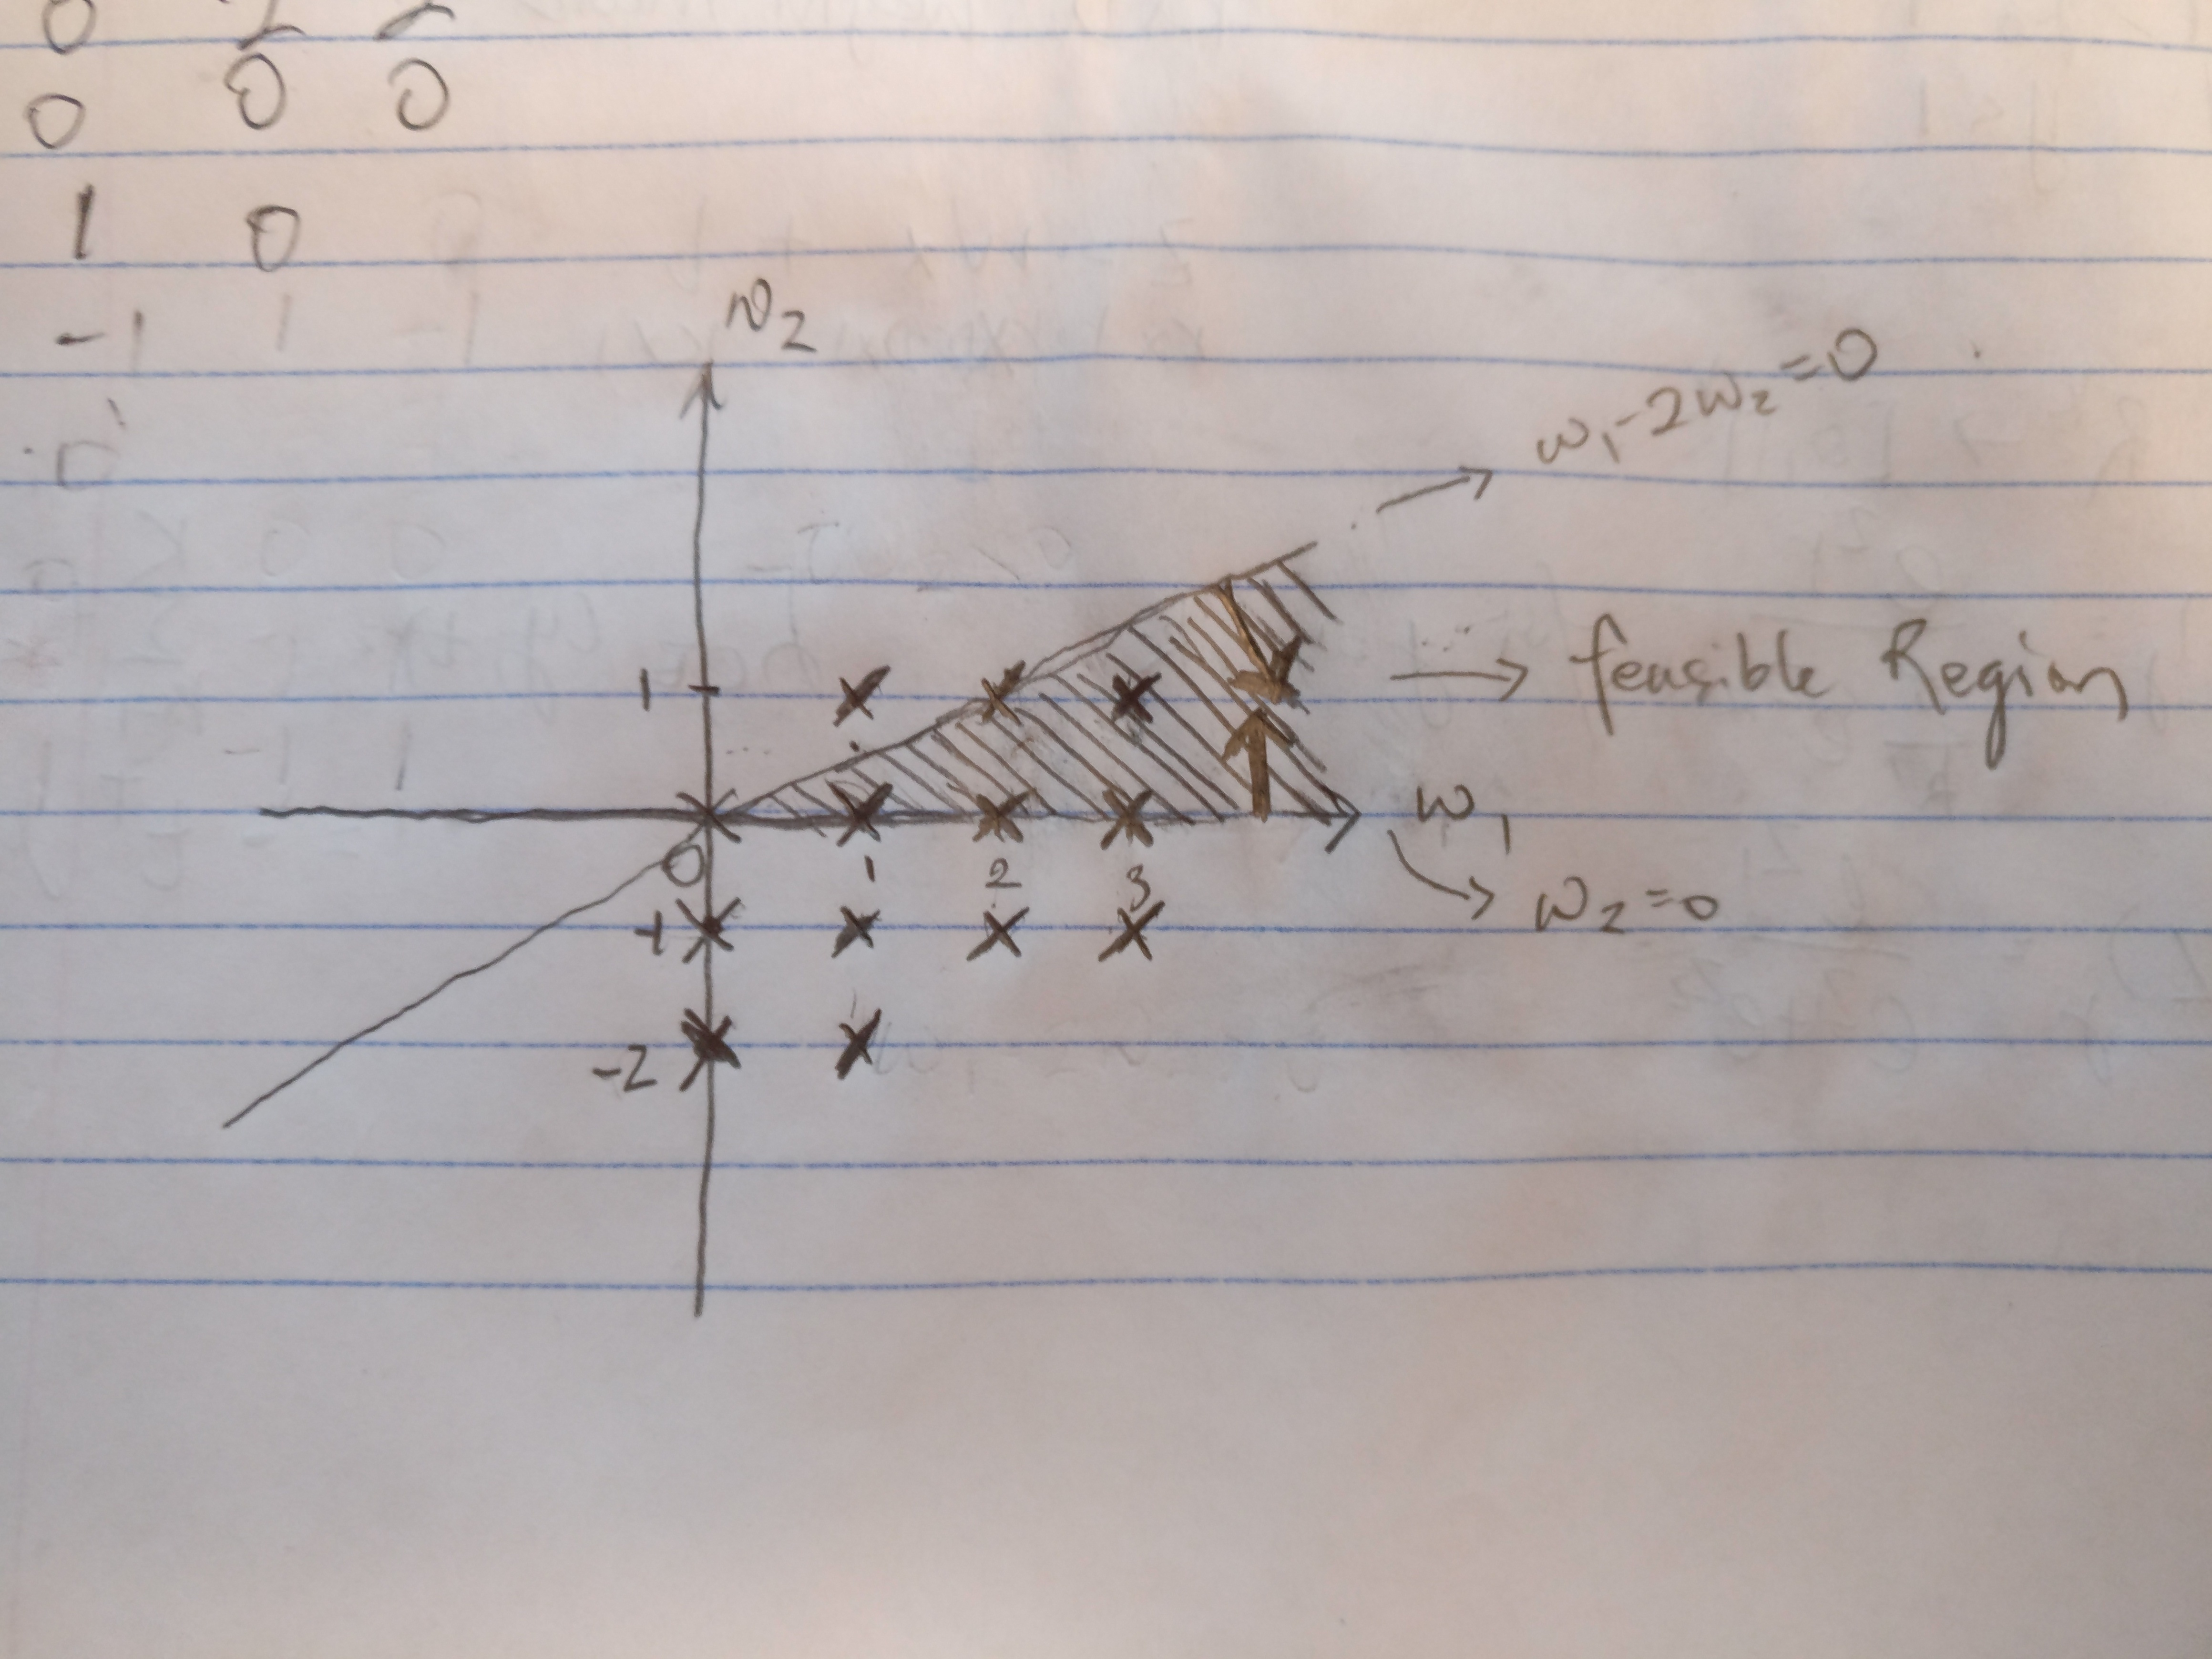
\includegraphics[width=10cm]{perceptrontrace.jpg}
\end{enumerate} 

\item \textbf{Feature Maps}  Suppose we have the following 1-D dataset for binary classification:


\begin{center}
    \begin{tabular}{ c | c }
     x & t \\ 
     \hline
     -1 & 1 \\  
     1 & 0 \\
     3 & 1 \\
    \end{tabular}
\end{center}

\begin{enumerate}
    \item Argue briefly (at most a few sentences) that this dataset is not linearly separable. Your answer should mention convexity. \\
    Note, we can write $x^{(2)}=1$ as a weighted average of $x^{(1)}$ and $x^{(3)}$, both of which lies in the convex positive region
    \[
        x^{(2)} = 1 = \frac{1}{2} \cdot -1 + \frac{1}{2} \cdot 3 = \lambda_1 x^{(1)} + \lambda_3 x^{(3)}
    \]
    where $\lambda_1 = \lambda_3 = \rfrac{1}{2}$ hence $\lambda_1, \lambda_3 > 0$ and $\lambda_1+\lambda_3 = 1$. Since $x^{(2)}$ is the weighted average of points in a convex set, it must also lie in the positive region. However, it is labelled as a negative example. Since we can't classify $x^{(2)}$ as both positive and negative, the problem must be linearly inseparable
    \item Now suppose we apply the feature map
    \[
        \boldsymbol{\psi}(x) = 
        \begin{pmatrix}
            \psi_1(x) \\ \psi_2(x)
        \end{pmatrix}
        = 
        \begin{pmatrix}
            x \\ x^2
        \end{pmatrix}
    \]
    Assume we have no bias term, so that the parameters are $w_1$ and $w_2$. Write down the constraint on $w_1$ and $w_2$ corresponding to each training exam- ple, and then find a pair of values $(w_1,w_2)$ that correctly classifies all the examples. Remember that there is no bias term.\\
    We can rewrite the dataset after applying the feature map 
    \begin{center}
        \begin{tabular}{c c | c}
            $\psi_1(x)$ & $\psi_2(x)$ & $t$ \\ 
            \hline
            -1 & 1 & 1 \\
            1 & 1 & 0 \\
            3 & 9 & 1 \\ 
        \end{tabular}
    \end{center}
    So we have constraints on $w_1$ and $w_2$ as follows 
    \[
        -w_1 + w_2 > 0 
        \quad \quad 
        w_1 + w_2 < 0
        \quad \quad 
        3w_1 + 9w_2 > 0
    \]
    $(w_1,w_2) = (-2,1)$ satisfies the constraints and so correctly classifies all examples
\end{enumerate}


\item \textbf{Loss Function} Suppose we have a prediction problem where the target $t$ corresponds to an angle, measured in radians. A reasonable loss function we might use is
\[
    \mathcal{L}(y,t) = 1 - \cos(y-t)    
\]
Suppose we make predictions using a linear model, 
\[
    y = \matr{w^Tx} + b     
\]
As usual, the cost is the average loss over the training set:
\[
    \mathcal{E} = \frac{1}{N} \sum_{i=1}^N \mathcal{L}(y^{(i)}, t^{(i)})    
\]
Derive vectorized expression for the following 
\begin{align*}
    \matr{y} &= \matr{Xw} + b\matr{1} \\
    \frac{\partial \mathcal{E}}{\partial \matr{y}} &= \frac{1}{N} \sin{(\matr{y - t})} \\
    \frac{\partial \mathcal{E}}{\partial \matr{w}} &= \frac{1}{N} \matr{X}^T \sin{(\matr{y-t})} \\ 
    \frac{\partial \mathcal{E}}{\partial b} &= \frac{1}{N} \matr{1}^T \sin{(\matr{y-t})} \\ 
\end{align*}
Some derivation steps are shown below 
\[
    \frac{\partial \mathcal{E}}{\partial y_j} = \frac{1}{N} \sin{(y^{(j)} - t^{(j)})}
    \quad \quad \rightarrow \quad \quad 
    \frac{\partial \mathcal{E}}{\partial \matr{y}} = \frac{1}{N} \sin{(\matr{y - t})} 
\]
\begin{align*}
    \frac{\partial \mathcal{E}}{\partial w_j} 
    &= \frac{\partial}{\partial w_j} \left(
        \frac{1}{N} \sum_{i=1}^N \left( 1 -\cos{\left(\sum_{j'=1}^D w_{j'}x_{j'}^{(i)} +b - t^{(i)} \right)} \right)    
    \right) \\ 
    &= \frac{1}{N} \sum_{i=1}^N x_j^{(i)} \sin{(y^{(i)} - t^{(i)})} 
    \quad \quad \rightarrow \quad \quad 
    \frac{\partial \mathcal{E}}{\partial \matr{w}} = \frac{1}{N} \matr{X}^T \sin{(\matr{y-t})}
\end{align*}
\[
    \frac{\partial \mathcal{E}}{\partial b} 
    = \frac{1}{N} \sum_{i=1}^N \sin{(y^{(i)} - t^{(i)})} 
    \quad \quad \rightarrow \quad \quad 
    \frac{\partial \mathcal{E}}{\partial b} = \frac{1}{N} \matr{1}^T \sin{(\matr{y-t})} 
\]






\end{enumerate}
\end{document}
